\section{Performance evaluation}

In this section, we want to evaluate our fluxionnal execution model to highlight its avantages and drawbacks.
We compare it based on the example described in the previous section, Figure \ref{fig:fluxions}.
This example is implemented in basic Javascript, listing \ref{lst:classique}, and in different fluxionnal execution models.

\subsection{Evaluation conditions}

We developed different fluxionnal execution models to test different instructions to chain fluxions implying different compromises.
Thus, through multiple implementations, we hope to compare the efficiency of the model itself, and erase the peculiarities brought by a single implementation.

Javascript itself doesn't feature an event loop, or a message queue.
However, as Javascript was historically used with DOM which makes use of an event loop, most of the Javascript interpreters - like \texttt{node.js} - now also feature an event loop.
The fluxionnal execution model is based around a message queue, so we used the event loop built inside \texttt{node.js} to act as the main message queue needed by the execution model.

There are different ways to queue messages in this event loop, they are depictured in firgure \ref{fig:eventloop}.
\begin{itemize}
	\item[\textit{function call}] doesn't use the event loop. It's the fastest way to continue execution, and it bypasses every IO.
	\item[\textit{process.nextTick}] queues a function just after the current execution. It bypasses IO.
	\item[\textit{setImmediate}] queues a function, doesn't bypass IO, but bypasses \textit{setTimeout}.
	\item[\textit{setTimeout}] queues a function, doesn't bypass IO is called with a certain latency.
\end{itemize}

\begin{figure}[h!]
  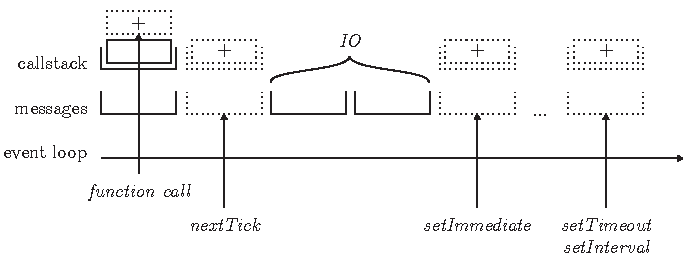
\includegraphics[width=\linewidth]{eventloop.pdf}
  \caption{Javascript event loop details}
  \label{fig:eventloop}
\end{figure}

We tested our model with three different implementations.

\begin{itemize}
	\item[\textbf{Chain}]
		This implementation chains fluxions one after another by a direct function call.
		The whole fluxion chain is contained inside a same stack on Figure \ref{fig:eventloop}.
		It sets the fluxions chain length maximum to the maximum function call stack size, and it's impossible to interleave messages from network in the middle of a fluxion chain.

	\item[\textbf{NextTick}]
		This implementation uses the instruction \texttt{process.nextTick} to chain fluxions execution.
		This instruction add a function call at the end of the current execution.
		Two local fluxion processing chains could run concurrently, but it's only possible to probe network messages every \textit{n} fluxions execution.
		By default \textit{n} is set to 1000.

	\item[\textbf{SetTimeout}]
		This implementation uses the instruction \texttt{setTimeout}.
		It probes network messages after every fluxion execution, thus networks messages can be interleaved between each local messages.
\end{itemize}

With these different implementations, we want to highlight the advantages and drawbacks of the fluxionnal execution model.

\subsection{Evaluation results}

% \begin{figure}
% \input{../../prototypes/fluxions/bench/charts/setTimeout}
% \caption{Response time for each implemetation in function of the number of simultaneous clients}
% \label{fig:setTimeout}
% \end{figure}

% \begin{figure}
% \input{../../prototypes/fluxions/bench/charts/distribution}
% \caption{Response time for each implemetation in function of the number of simultaneous clients}
% \label{fig:timecountsetTimeout}
% \end{figure}

As we can see on Figure \ref{fig:distribution}, the difference between the basic implementation and the chained implementation is insignificant, we can conclude that splitting a web service into fluxions doesn't induce significative performance loss.
And even the implementation using \texttt{nextTick} is almost as efficient as the basic implementation.
However, the implementation using \texttt{setTimeout} is about 5 times less efficient than the basic implementation.

\TODO{}
Although, using a fluxionnal approach is a way to build an efficient distributed system we consider that the most important part of our work is to enable code transformation from a standard basic web approach to a flow of fluxions.
We show now the main code transformation we propose.